\documentclass[]{standalone}
\usepackage{tikz}
\usetikzlibrary{shapes,arrows,calc,positioning}
\usepackage{amsmath} % for dfrac
\usepackage{comment}
\usepackage{calc}

% definition of basic block
\tikzset{
    block/.style = {draw, rectangle,
        minimum height=1.2cm,
        minimum width=2cm},
    input/.style = {coordinate,node distance=1cm},
    output/.style = {coordinate,node distance=1cm},
    sum/.style = {draw, circle, node distance=1cm},
}

% definition of saturation block
\tikzset{% from https://tex.stackexchange.com/questions/161075/saturation-block
  saturation block/.style={%
    draw, 
    path picture={
      % Get the width and height of the path picture node
      \pgfpointdiff{\pgfpointanchor{path picture bounding box}{north east}}%
        {\pgfpointanchor{path picture bounding box}{south west}}
      \pgfgetlastxy\x\y
      % Scale the x and y vectors so that the range
      % -1 to 1 is slightly shorter than the size of the node
      \tikzset{x=\x*.4, y=\y*.4}
      %
      % Draw annotation
      \draw (-1,0) -- (1,0) (0,-1) -- (0,1); 
      \draw (-1,-.7) -- (-.6,-.7) -- (.6,.7) -- (1,.7);
    }
  }
}
\tikzset{% from https://tex.stackexchange.com/questions/161075/saturation-block
  deadband block/.style={%
    draw, 
    path picture={
      % Get the width and height of the path picture node
      \pgfpointdiff{\pgfpointanchor{path picture bounding box}{north east}}%
        {\pgfpointanchor{path picture bounding box}{south west}}
      \pgfgetlastxy\x\y
      % Scale the x and y vectors so that the range
      % -1 to 1 is slightly shorter than the size of the node
      \tikzset{x=\x*.4, y=\y*.4}
      %
      % Draw annotation
      \draw (-1,0) -- (1,0) (0,-1) -- (0,1);  % axis
      \draw (-1,1) -- (-.3,.3) -- (-.3,0) -- (.3,0) -- (.3,-.3) -- (1,-1);
	  %\draw (-.3,.3) -- (.3,-.3) ;
    }
  }
}

\begin{document}
	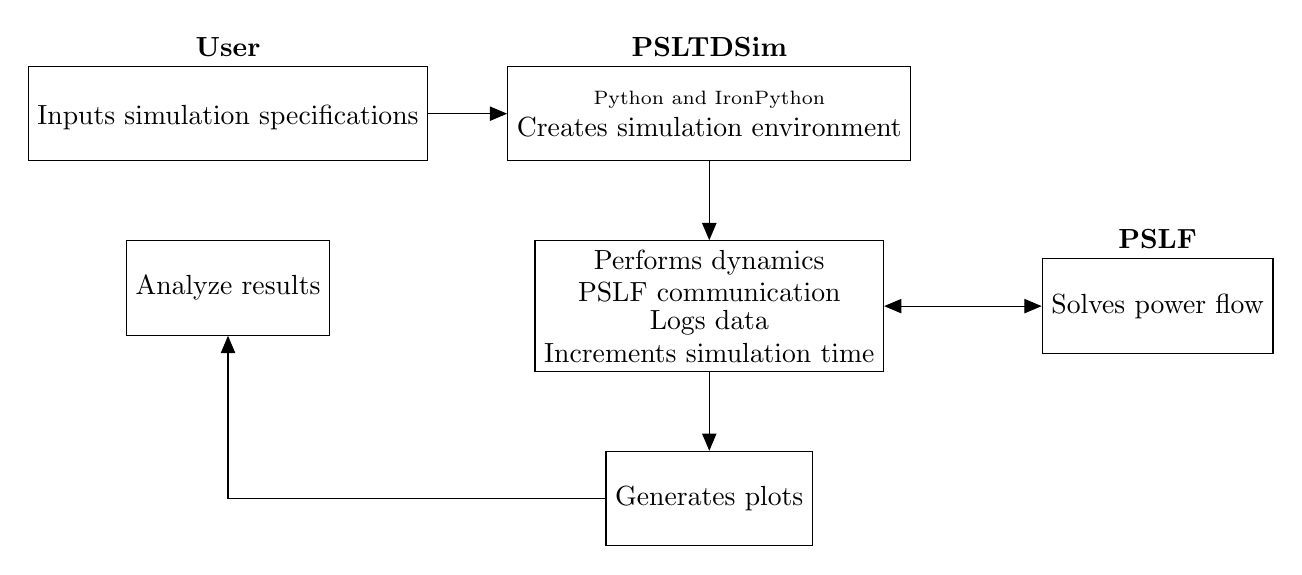
\begin{tikzpicture}[auto, node distance=1cm,>=triangle 45]
		
		
		% user
		\node [block, label=\textbf{User}] (user) {\shortstack{\\ Inputs simulation specifications}};
		\node [block, below= of user] (userout) {\shortstack{Analyze results}};
		
		% python init
		\node [block, right=of user,label=\textbf{PSLTDSim} ] (python) {\shortstack{{\scriptsize Python and IronPython}\\ Creates simulation environment}};
		% python loop
				\node [block, below=of python,] (pythonloop) {\shortstack{Performs dynamics\\ PSLF communication\\ Logs data\\ Increments simulation time}};
		% python output
				\node [block, below=of pythonloop,] (pythonoutput) {\shortstack{Generates plots}};
		
		% pslf
		\node [block, right=2cm of pythonloop, label=\textbf{PSLF} ] (pslf) {\shortstack{Solves power flow}};
		

		\draw [->] (user) -- (python);
		\draw [->] (python) -- (pythonloop);
		\draw [<->] (pythonloop) -- (pslf);
		\draw [->] (pythonloop) -- (pythonoutput);
		\draw [->] (pythonoutput) -| (userout);

	\end{tikzpicture} 
\end{document}